% !TEX root = ../../prj4projektdokumentation.tex

\section{Belastning}

Med denne distributionslinje og med trinskifteren, der står på 4V trinnet, kan det beregnes hvilken belastning, der vil medføre, at spændingen hos forbrugeren falder til under 10 \% \\ af 4V. Kredsløbet og beregningen ses nedenfor.

\begin{figure}[htbp] % (alternativt [H])
	\centering
	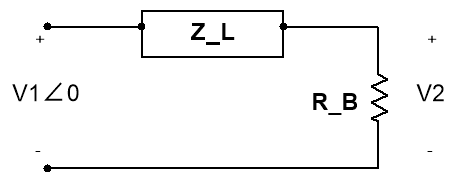
\includegraphics[width=0.4\textwidth]{Figure/Belastningberegning}
	\caption{Kredsløb til beregning af belastning}
	\label{fig:Belastningberegning}
\end{figure}

Først bruges spændingsdelerformlen

\begin{align}
	V2=V1\cdot\frac{R_B}{Z_L+R_B}
\end{align}

\begin{align}
	0,9\cdot\vert V1 \vert = \vert V1\cdot\frac{R_B}{Z_L+R_B} \vert = V1\cdot\frac{R_B}{R_L+jX_L+R_B}
\end{align}

\begin{align}
0,9= \vert \frac{R_B}{R_L+jX_L+R_B} \vert
\end{align}

\begin{align}
	0,9\cdot\vert R_L+jX_L+R_B \vert = \vert R_B \vert
\end{align}

\begin{align}
0,9\cdot\sqrt{(R_L+R_B)^2+X_L^2}=R_B
\end{align}

\begin{align}
(R_L+R_B)^2+X_L^2=\frac{R_B^2}{0,81}
\end{align}

\begin{align}
R_L^2+R_B^2+2\cdot R_L\cdot R_B+X_L^2=\frac{R_B^2}{0,81}
\end{align}

\begin{align}
R_B^2\cdot (1-\frac{1}{0,81})+2\cdot R_L\cdot R_B+X_L^2=0
\end{align}

Værdier indsættes og herved fås:

\begin{align}
R_B^2\cdot (-0,24) +12,4\cdot R_B+18,23=0
\end{align}

Andengrads ligning løses og derved findes den modstandsværdi, der vil give et spændingsfald på 10\%.

\begin{align}
R_B=\frac{-12,4\pm\sqrt{153,76-4\cdot(-0,24)\cdot18,23}}{-0,24\cdot 2}=\frac{-12,4\pm 13,1}{-0,47}=54,3 \Omega
\end{align}

Denne modstandsværdi i det viste kredsløb og med den valgte distributionslinje vil resultere i at spændingen falder under det øsnkede niveau som er 4V. Der tages derfor udgangspunkt i denne værdi, men efterfølgende vil belastninger bestemmes ud fra simuleringer i værktøjet Multisim. 



